\documentclass{tufte-handout}

\title{On ultimate; O1: primary middle, focus or left wing}
\author[James Reynolds]{James Reynolds}

%\date{28 March 2010} % without \date command, current date is supplied

%\geometry{showframe} % display margins for debugging page layout

\usepackage{graphicx} % allow embedded images
  \setkeys{Gin}{width=\linewidth,totalheight=\textheight,keepaspectratio}
  \graphicspath{{graphics/}} % set of paths to search for images
\usepackage{amsmath}  % extended mathematics
\usepackage{booktabs} % book-quality tables
\usepackage{units}    % non-stacked fractions and better unit spacing
\usepackage{multicol} % multiple column layout facilities
\usepackage{lipsum}   % filler text
\usepackage{fancyvrb} % extended verbatim environments
  \fvset{fontsize=\normalsize}% default font size for fancy-verbatim environments

% Standardize command font styles and environments
\newcommand{\doccmd}[1]{\texttt{\textbackslash#1}}% command name -- adds backslash automatically
\newcommand{\docopt}[1]{\ensuremath{\langle}\textrm{\textit{#1}}\ensuremath{\rangle}}% optional command argument
\newcommand{\docarg}[1]{\textrm{\textit{#1}}}% (required) command argument
\newcommand{\docenv}[1]{\textsf{#1}}% environment name
\newcommand{\docpkg}[1]{\texttt{#1}}% package name
\newcommand{\doccls}[1]{\texttt{#1}}% document class name
\newcommand{\docclsopt}[1]{\texttt{#1}}% document class option name
\newenvironment{docspec}{\begin{quote}\noindent}{\end{quote}}% command specification environment

\begin{document}

\maketitle% this prints the handout title, author, and date



%\printclassoptions
This is 
a two-pager 
on being 
primary middle, 
the focus, 
or left wing 
on offence. 
It is  
referred to here 
as position O1\footnote{
This
is part of a series, 
available at
\url{https://github.com/James-Reynolds/Ultimate-strategy-and-tactics}.}.


\section{Beating person-match defence with a vertical stack}\label{sec:vertical}

\begin{marginfigure}%
  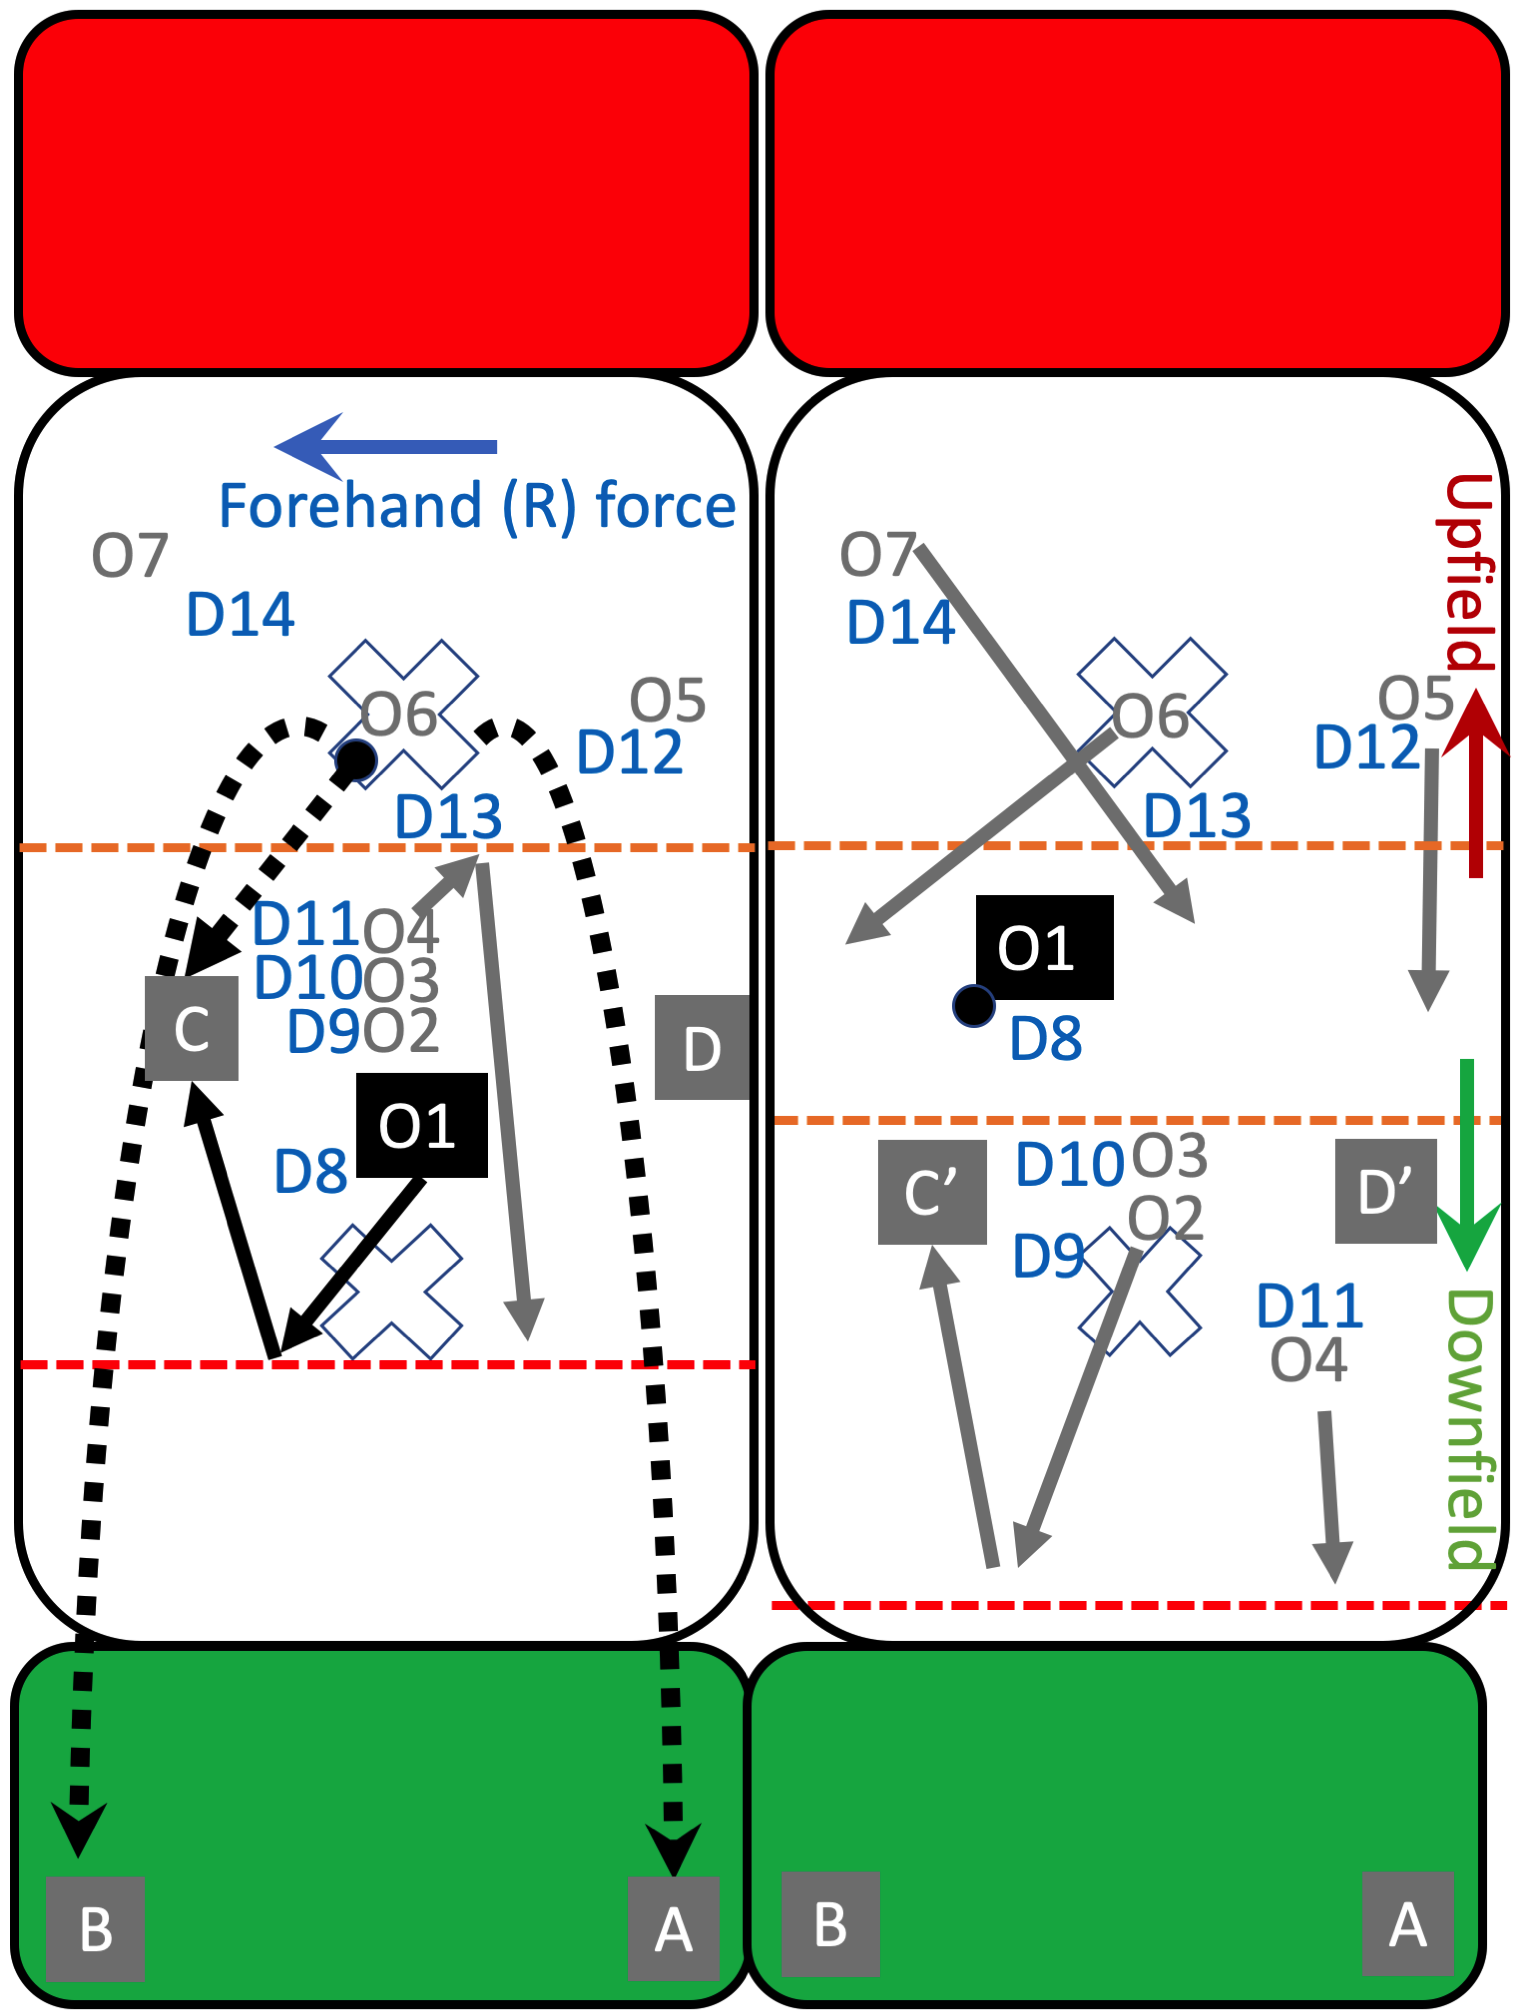
\includegraphics[width=\linewidth]{O1-vertical}
  \caption{Vertical stack: 
  starting position (left),
  and development (right)}
  \label{fig:O1-vertical}
\end{marginfigure}


Figure \ref{fig:O1-vertical} (left) shows 
a situation 
with 
your team: 
using 
a vertical stack formation; 
having called a brick; and
facing a 
forehand force with 
person-match defence\footnote{
Vertical works
against other person-match defences, 
but might need 
adjustment e.g. 
(1) RH-backhand-force: mirror everything;
(2) straight up force, 
wait while handlers 
move it about 
until they can huck 
to you (going to A or B);
(3) last-person-covers-deep,
coordinate with O2 
to overload D8 (deep) 
or D9 (under); etc.}. 
O6 is shown
potentially throwing 
you (O1):
\begin{enumerate}
\item A break-side 
huck to A.
This throw is 
probably 
difficult. 
However, you as O1
can just
stand still 
till O6 throws it, 
then run and catch it.
D8 will be on the wrong side of you
and so probably 
not be able 
to get to the disc
first.
\item An open-side huck to B. 
This is viable if: 
D8 is closer to the disc than you; 
you are faster than D8; or 
D8 does not cover 
an initial cut downfield (black arrow). 
\item A throw 
to C.
The solid black arrows indicate 
a cut you might do;
initially going deep,
but then coming back-under
on the open side. 
\item A break to D. 
You can stand still 
and run onto this one 
once it is thrown 
as D8 is already on 
the wrong side to intercept 
this throw. 
\end{enumerate}
When cutting,
staying  
between 
the dashed 
horizontal 
lines 
may help\footnote{ 
The position of 
the lines vary
with the position of the disc
and with how far the thrower  
can or will 
throw.}. 
If you go 
downfield of the dashed red line 
before the disc is in the air,
D8 (your marker) 
may be able 
get to
A or B 
before the disc,
intercepting 
or preventing
any deep throws\footnote{
To you, 
or anyone else.
By going 
too far 
from the disc 
you 
effectively
allow your marker 
to poach deep.}.
Similarly, 
if you go 
upfield of the dashed yellow line
then D8 
might help
prevent dumps.

Figure \ref{fig:O1-vertical} (right) shows 
the disc having been thrown to you
on the back-under cut towards C. 
In order of desirability, 
your options may include: 
(1)
off-load to O6, 
putting them in power position\footnote{
Because D13 
will likely be trailing them 
and O6 
will be looking downfield 
as they catch the disc, 
they can
then pretty much 
throw to anywhere.};
(2) throwing to A' to hit O2 or O4;
(3) throwing to B' or C' for O2;
(4) break force throw 
to centre the disc
to O3 or O5;
(5) dump to O7, then
head back to the stack, 
or make another cut.

\subsection{Beating person-match defence with feldrunner}
\label{sec:feld}
Figure \ref{fig:O1-horizontal} (left) 
shows a feldrunner formation, 
with 4 handlers, 
2 cutters 
in the endzone,
and you 
(O1) 
left  
isolated 
in the centre
as the focus. 
O6 can throw 
to A,
B, 
C 
or D. 
If D8 looks at you, 
stand still and 
O6 can throw it 
to your advantage. 
If D8
looks at O6, 
cut to A-D. 
Instead, 
O6 might reset 
to O4, O5 or O7, 
for them to 
throw to you. 
With the disc 
you can throw
to cuts from O2-3, 
or dump and repeat. 

\begin{marginfigure}%
  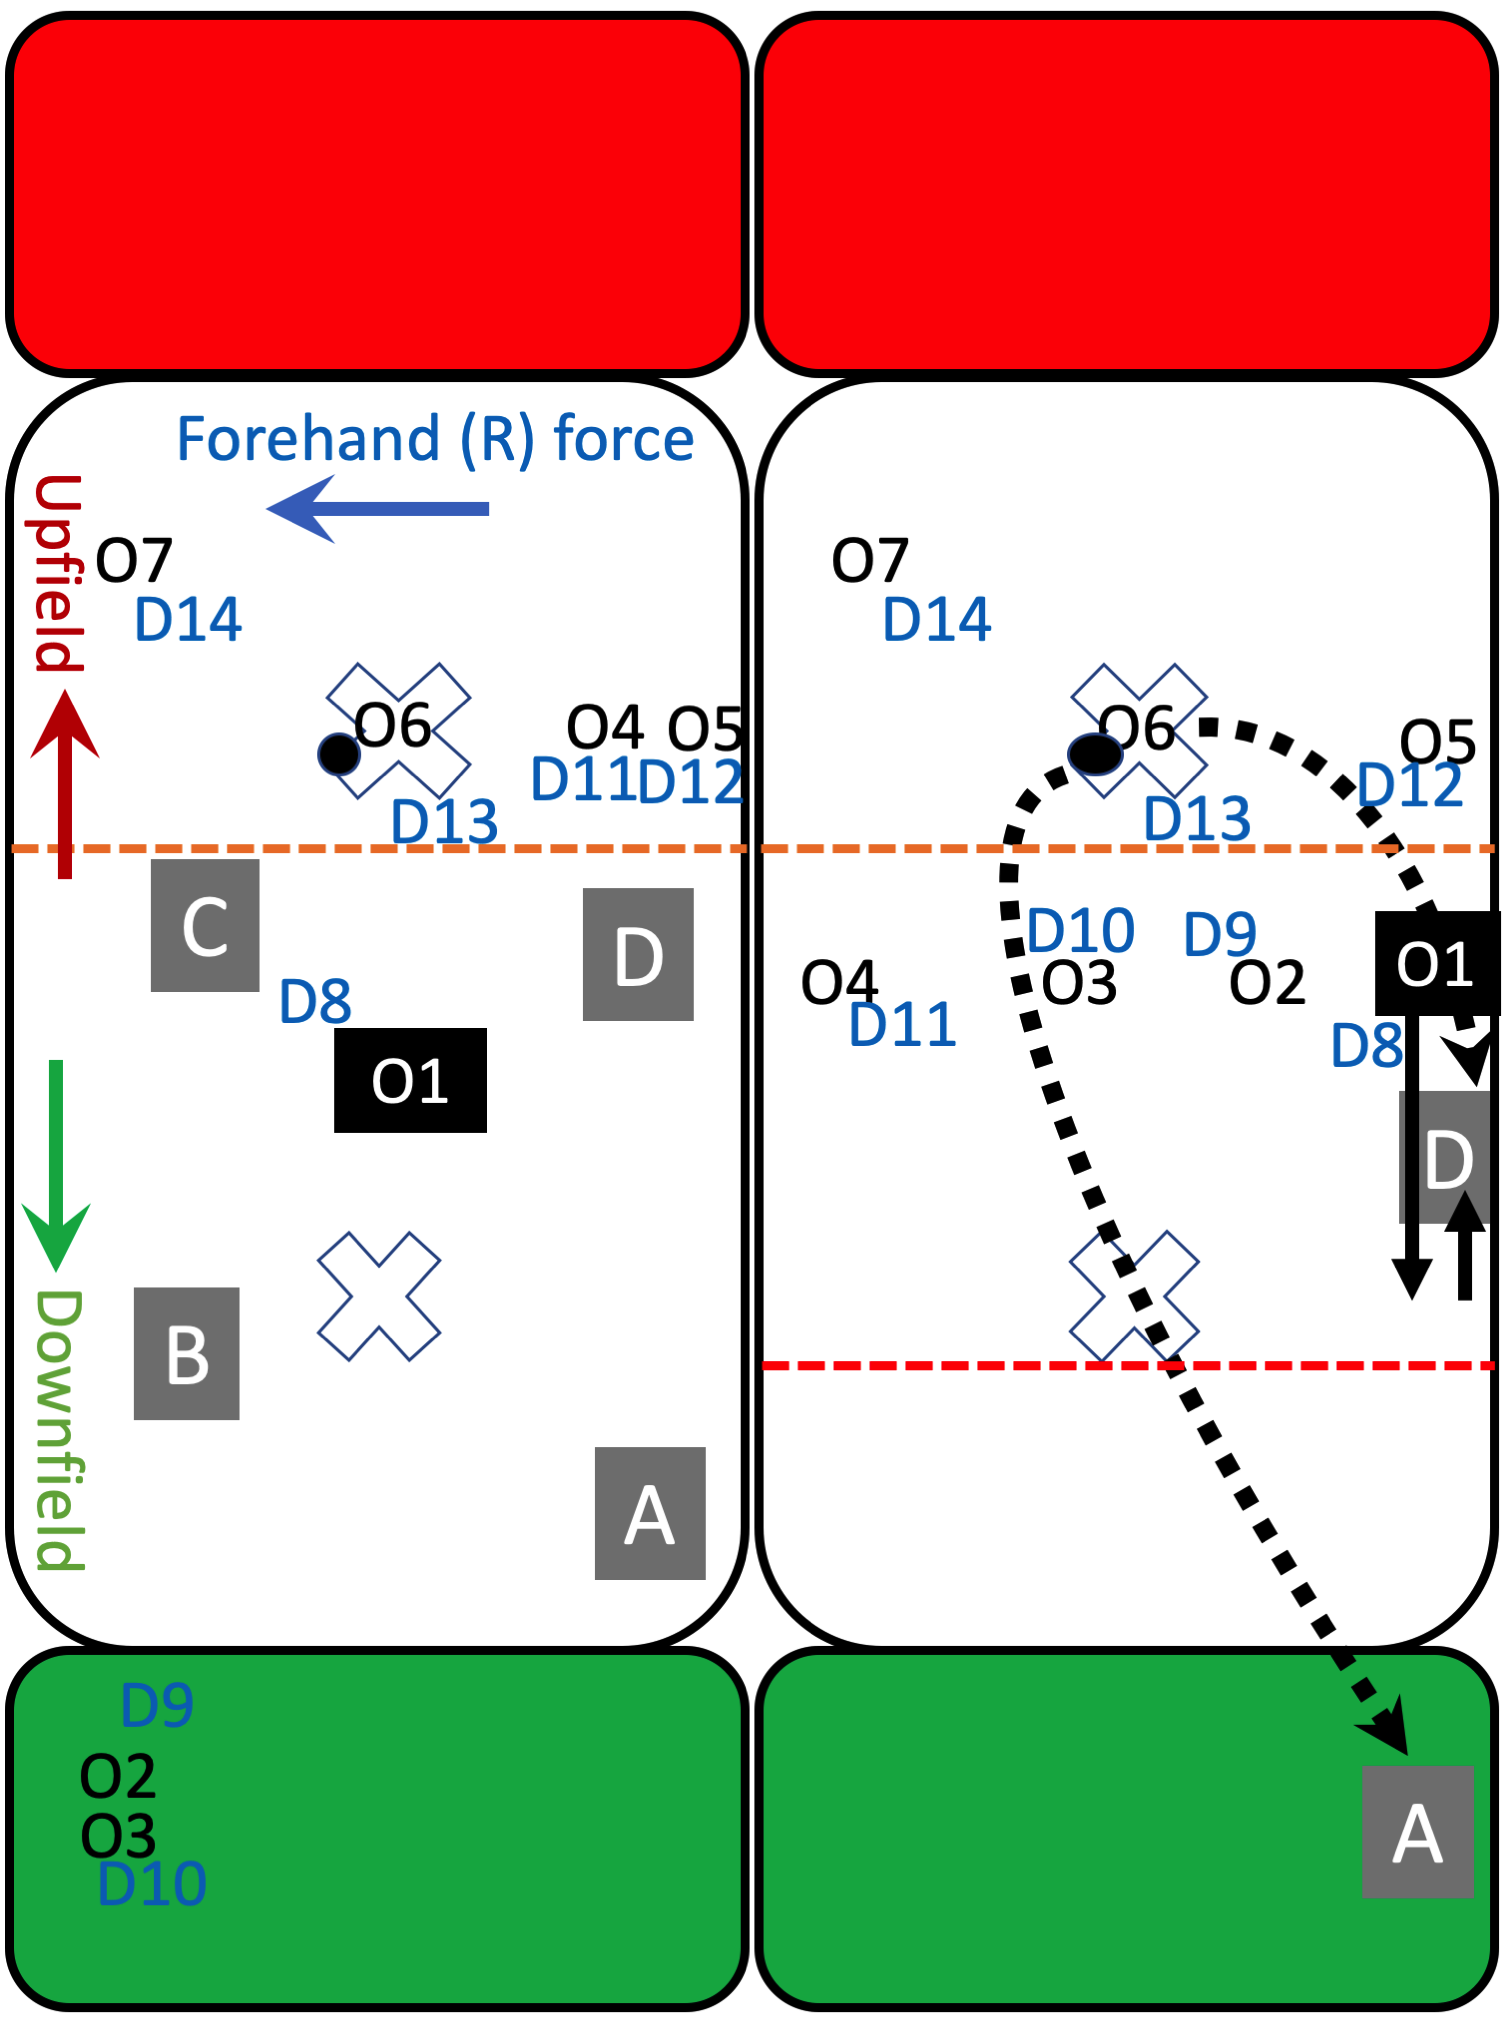
\includegraphics[width=\linewidth]{O1-horizontal}
  \caption{Feld (left) and ho-ro (right)}
  \label{fig:O1-horizontal}
\end{marginfigure}


\subsection{Beating person-match defence with a horizontal stack}\label{sec:horizontall}
Figure \ref{fig:O1-horizontal} (right) shows 
you (O1) 
on the left wing. 
This formation 
typically involves cutting
upfield and downfield (black arrows)
within your quarter of the field\footnote{
Other cuts
can work, 
but might need
communication,
e.g. diamond cuts 
involve you trading places 
with O2.}. 
O6 
can potentially 
throw to you 
at A 
or D\footnote{
Black arrows
show how a back-under cut 
opens space 
for this throw.}. 
However, 
O6 throwing to 
O2, O3 or O4  
may be easier. 
Hence,  
you may wish to 
wait and 
cut later. 
If you do get the disc 
at D 
a huck to 
A for O2 or 
to B for O4 
may be effective.
Otherwise, 
get it to the middle of the field 
with a dump to O5 or O6. 

A typical pattern
is that D8 (marking you)
will try to help 
D9, D10 and D11 
by poaching deep.
To beat this 
you can: 
trade spots with O5;
move to the open side, 
between D10 and O6; or 
stay still 
on the left wing,
so O6 can 
get it to you 
quickly
with a hammer 
or blade.

\section{Beating zone defence}\label{sec:zone}

\begin{marginfigure}%
  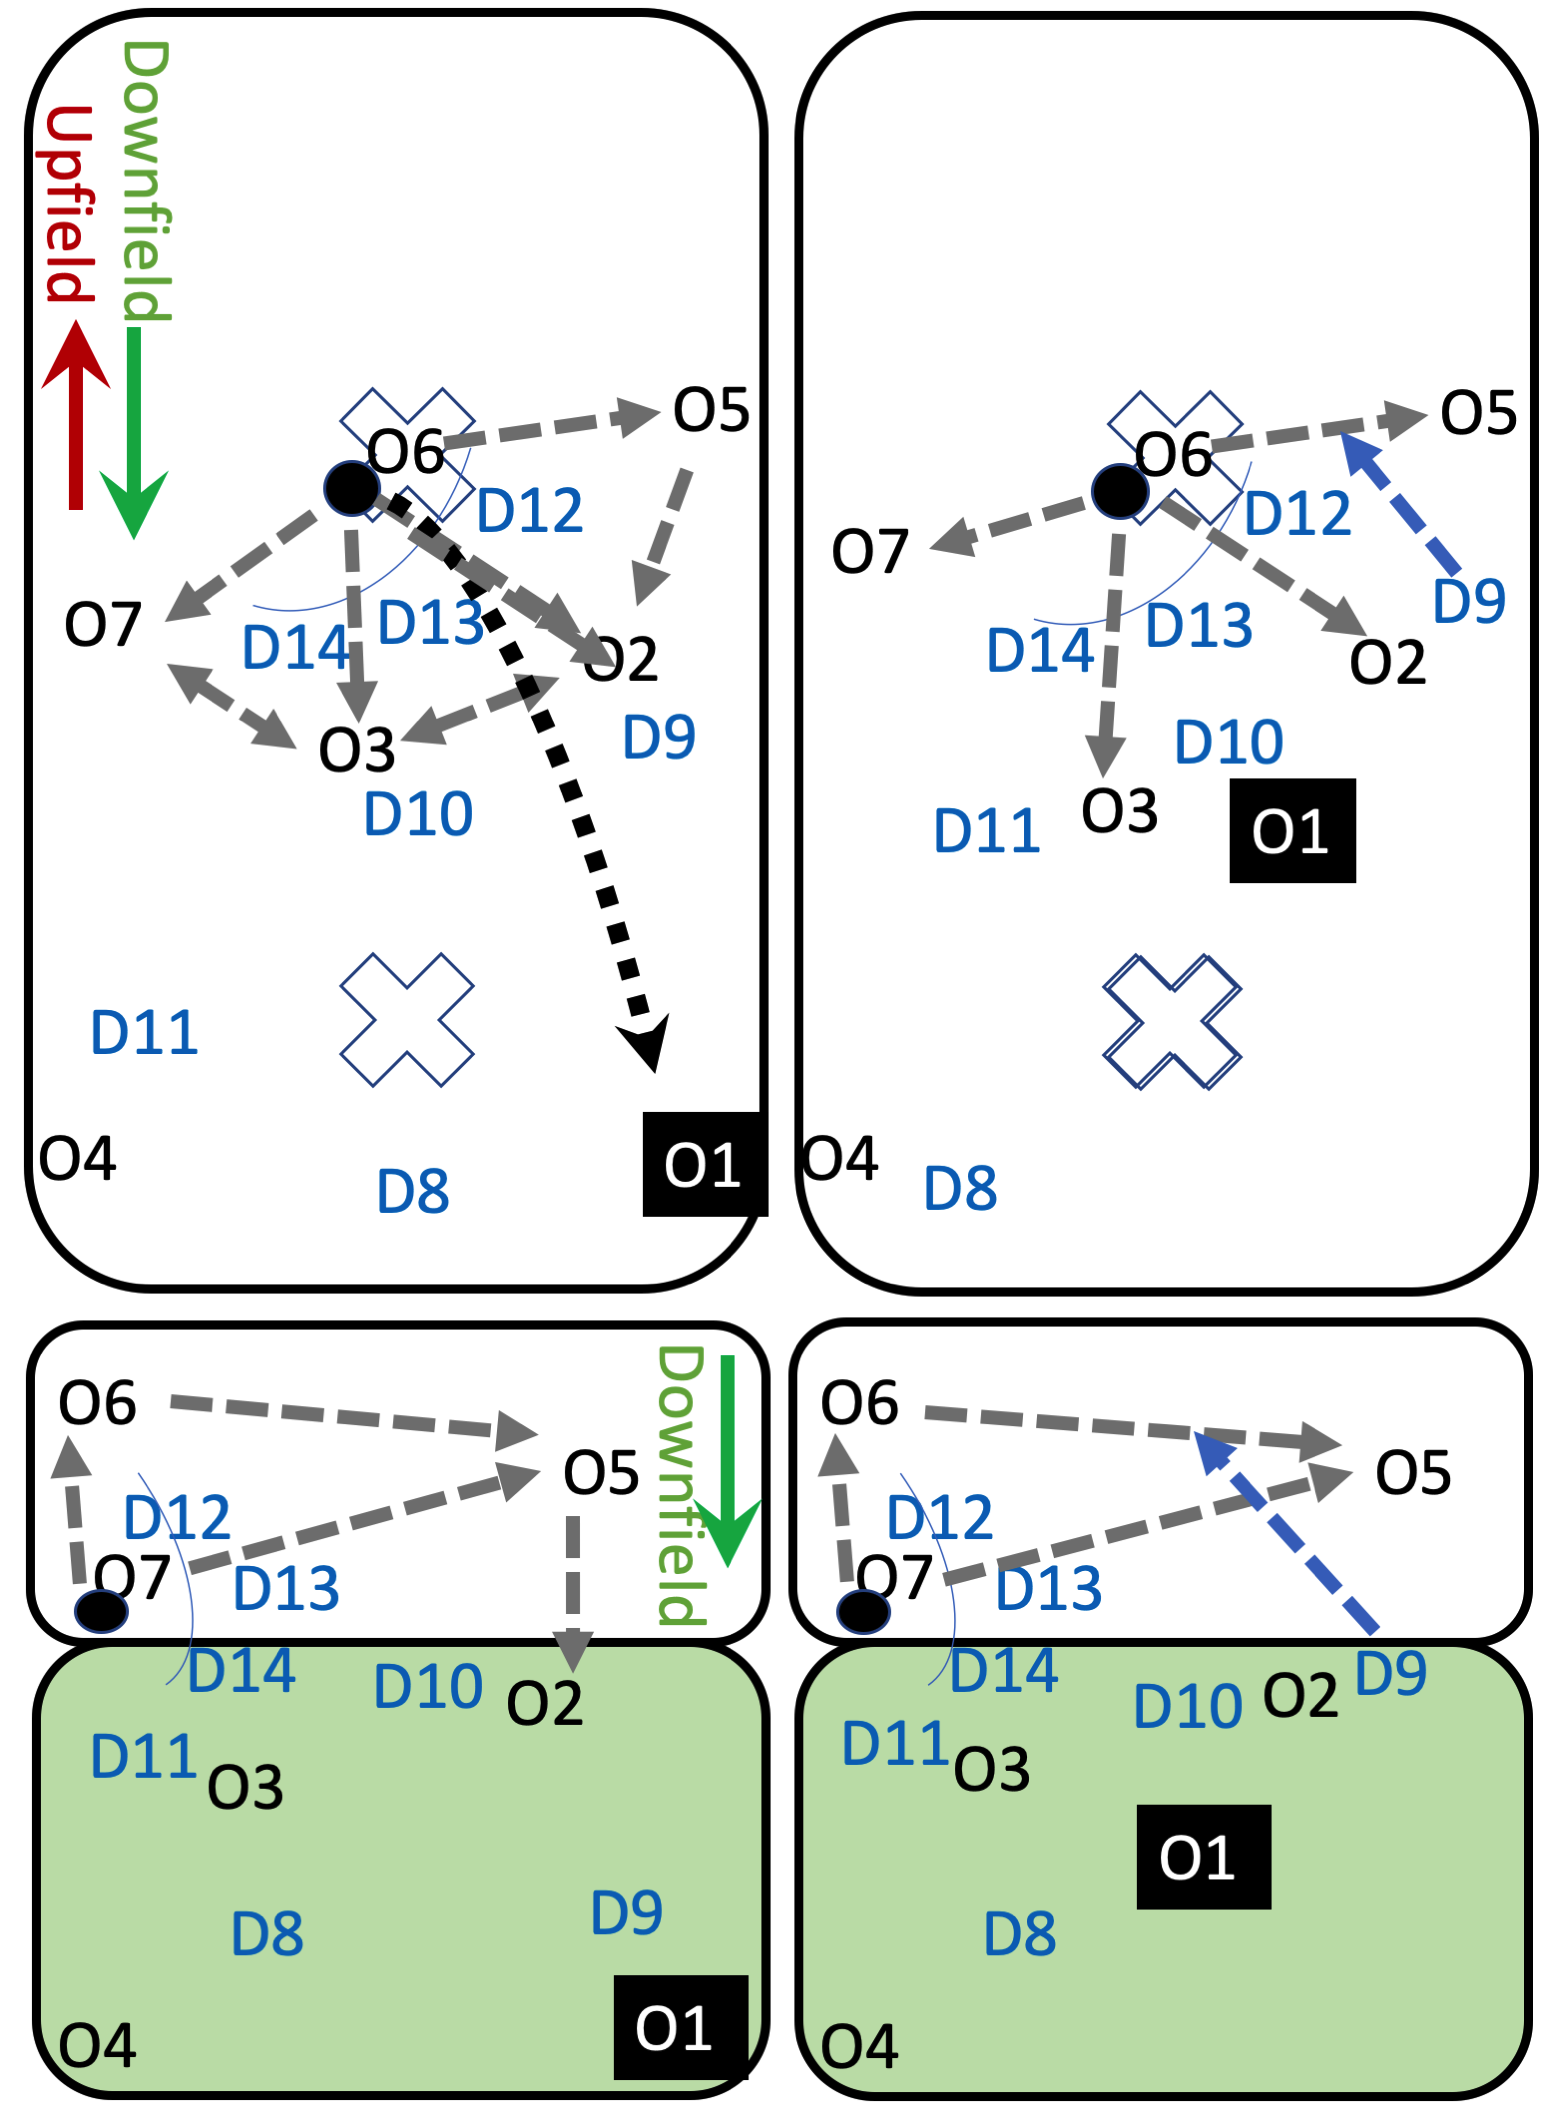
\includegraphics[width=\linewidth]{O1-zone331}
  \caption{effective formations against 331 zone: 
  general (top left)
  and close to the endzone (bottom left); and 
  less effective formations (top, bottom right)}
  \label{fig:O1-zone331}
\end{marginfigure}

Vertical stack 
probably won't work. 
Instead, your 
team needs to 
spread out. 
Three ways to beat a zone are:
(1) over;
(2) round; or
(3) through. 
Figure \ref{fig:O1-zone331}
(top left)
shows this 
against a 
3-3-1 zone, 
with a throw 
direct 
from O6 
\smallcaps{over} to you\footnote{
This may be a 
blade or
hammer, 
to get it 
to you
as quickly as possible.
So it may help to 
stand still 
and look at O6.}.
Otherwise, 
O6 might throw
over or through (to O2 or O3), 
or round (to O5 or O7)\footnote{
You, 
O2, 
O3 and
O5
might then split
D9-10
to make ground 
before the cup 
(D12-14) catch up. 
Once they do, 
dump to O6 
so all 7 of your players
are involved again.}. 

If the defence 
continues to play zone 
once the disc 
gets close to the endzone, 
you (O1) 
and the other wing (O4) 
can \smallcaps{go and stand 
on the back corners}
(Figure \ref{fig:O1-zone331} (bottom left)\footnote{ 
The defence 
will either  
leave you open,
or cover you
at the corner
(D8 
or D9), 
making more space 
for O2, 
O3 and
O5-7 
at the front of the endzone.}.
Figure \ref{fig:O1-zone331} (bottom right) shows 
how the further 
you are from the back corner 
the more D8/9 
can cover both you
AND others,, 
and the harder 
it is to throw direct to you.
D9 might even be able to get a block
on a throw to O5
(dashed blue line). 
This applies also when 
not close to the endzone 
(top right).
If you crowd forward,
D8 only has to cover O4, 
and D9-11 
can push upfield.


\section{Beating clam defence}\label{sec:zone}
Clam mixes person-match 
and zone defence styles, 
with defenders 
switching frequently.
%\footnote{
%For example, 
%in Figure \ref{fig:O2-vertical}(left) 
%D8 
%might cover 
%O1 deep, 
%switching later 
%(with D9 or D11
%to cover O4's cut deep,
%rather than following O1 
%upfield to C.}. 
You might
coordinate 
with others  
to overload 
a defender, 
or spread out 
to give the handlers 
space 
and targets deep. 

\newthought{...and finally} 
this is just a two pager; 
there are many more 
offensive strategies 
and tactics\footnote{
Try 
a side stack. 
Similar to vertical, 
but with your stack 
hard up against 
one of the sidelines. 
This reduces the risk of picks, 
changes cutting angles, 
and provides space 
to make a cut going across 
the field, only to turn back 
and receive 
a disc thrown 
behind you.}
Remember, 
defence wins games, 
offence loses them\footnote{
Least turnovers 
usually wins.} 
and after a turnover 
it's better to get it back 
with another turnover, 
than receiving another pull!

\end{document}
